\documentclass[landscape,a0paper,blockverticalspace = 5mm]{tikzposter}

\usepackage[english]{babel}
\usepackage{amsmath, amsfonts}
\usepackage{fontspec}
\usepackage{unicode-math}
\usepackage{svg}

%\usefonttheme{professionalfonts} % Otherwise a bunch of DeclareMathOperator stuff breaks. There's something on TeX SE somewhere.
\setmainfont[Ligatures=TeX]{TeX Gyre Pagella}   % This probably needs tweaking.
\setmathfont{TeX Gyre Pagella Math}
\setmathfont[range=\symcal]{Asana Math}
\setmathfont[range=\setminus]{Asana Math}
%\newfontfamily\DejaVuSans{DejaVu Sans} % For unicode smileys.

\usepackage{microtype}

\usepackage{graphicx}
\usepackage{url}
\usepackage{enumitem}
\usepackage{csquotes}
%\usepackage[hidelinks=true]{hyperref}
\usepackage{tikz}
\usetikzlibrary{cd, calc, shapes, decorations.shapes, decorations.markings, decorations.pathreplacing, shapes.geometric, shapes.symbols}
\usepackage{tikz-cd}
\usepackage{blindtext}

\usepackage[backend=biber,doi=false,style=numeric,maxnames=2,maxbibnames=9]{biblatex}
%\bibliography{bibliography.bib}
%\bibliographystyle{plain}
\renewcommand*{\bibfont}{\scriptsize}

\DeclareMathOperator{\linspan}{span}
\DeclareMathOperator{\im}{im}
\newcommand{\myfix}[1]{{\color{red}(#1)}}
\newcommand{\myciteauthor}[1]{\citeauthor{#1}~\cite{#1}}
\newcommand{\myciteauthorshort}[1]{\citeauthor{#1},~\citeyear{#1}}
\newcommand{\myciteauthoryear}[1]{\citeauthor{#1}~\citeyear{#1}~\cite{#1}}
\newcommand{\defword}[1]{\emph{#1}}
\newcommand{\ZZ}{\ensuremath{\mathbb{Z}}}
\newcommand{\RR}{\ensuremath{\mathbb{R}}}
\newcommand{\NN}{\ensuremath{\mathbb{N}}}
\newcommand{\lap}{\ensuremath{\mathcal{L}}}
\newcommand{\lapu}{\ensuremath{\mathcal{L}^{\text{up}}}}
\newcommand{\lapd}{\ensuremath{\mathcal{L}^{\text{down}}}}
\newcommand{\fourier}{\ensuremath{\mathcal{F}}}

\newcommand{\ip}[2]{\ensuremath{\left\langle #1 , #2 \right\rangle}}
\newcommand{\ie}{}
\def\ie/{i.e.}
\newcommand{\eg}{}
\def\eg/{e.g.}
\newcommand{\etc}{}
\def\etc/{etc.}
\newcommand{\wrt}{}
\def\wrt/{wrt.}
\newcommand{\suchthat}{\ensuremath{\, \mid \,}}
\newcommand{\iso}[0]{\ensuremath{\cong}}

\newcommand{\placeholderfigure}[2]{\begin{tikzpicture}
    \draw[help lines,step=1cm] (0, 0) grid (#1 cm, #2 cm);
    \pgfmathsetmacro{\midx}{#1/2}
    \pgfmathsetmacro{\midy}{#2/2}
    \node[text width=#1 cm, align=center] () at (\midx cm,\midy cm) {PLACEHOLDER (#1 cm $\times$ #2 cm à cm unit grid)};
  \end{tikzpicture}
}
\definecolor{dgreen}{rgb}{0.0, 0.5, 0.0}
\tikzset{twosimp/.style={fill opacity=0.3,fill=blue,draw opacity=0.7}}
\tikzset{twosimp_red/.style={fill opacity=0.1,fill=dgreen,draw opacity=0.6}}
\tikzset{twosimp_yellow/.style={fill opacity=0.4,fill=dgreen!80!black,draw opacity=0.6}}
\tikzset{twosimp_orange/.style={fill opacity=0.5,fill=dgreen!80!black,draw opacity=0.6}}
\tikzset{twosimp_orangedark/.style={fill opacity=0.6,fill=dgreen,draw opacity=0.6}}
\tikzset{twosimp_green/.style={fill opacity=0.7,fill=dgreen!70!black,draw opacity=0.6}}
\tikzset{twosimpred/.style={fill opacity=0.3,fill=red,draw opacity=0.2}}
\tikzset{threesimp/.style={fill opacity=0.8,fill=dgreen!60!black,draw opacity=0.9}}
\tikzset{belowdiag/.style={fill opacity=0.2,fill=gray,color=gray, draw opacity=0.6}}



\newtheorem{thm}{Theorem}[section]
\newtheorem{obs}{Observation}[section]

% https://tex.stackexchange.com/questions/167521/tikz-poster-aligning-titlegraphic-to-the-right-of-the-title
\makeatletter
\renewcommand\TP@maketitle{%
   \begin{minipage}{0.6\linewidth}
        \centering
        \color{titlefgcolor}
        {\bfseries \Huge \sc \@title \par}
        \vspace*{1em}
        {\Large \@author \par}
        \vspace*{1em}         % Put back in if there's an institute line.
        {\LARGE \@institute}  %
    \end{minipage}%
   %\hfill
   \hspace{5em}
    \begin{minipage}{0.4\linewidth}
      \vspace*{0em}
       %\centering
       \@titlegraphic
    \end{minipage}
}
\makeatother

\title{\parbox{\linewidth}{ \centering Simplicial Neural Networks}}

\author{Stefania Ebli, Micha\"{e}l Defferrard, Gard Spreemann}
%\institute{Laboratory for Topology and Neuroscience (Prof.\ Kathryn Hess)}

\titlegraphic{
\includegraphics[height=6em]{figures/EPFL_Logo_Digital_BLACK_PROD.png} }


\usetheme{Basic} % Wave is also decent.
\usecolorpalette{BlueGrayBlue}%{GreenGrayViolet} % Default,


\begin{document}
\maketitle

\begin{columns}

  \column{0.5}{

    \block{Convolution: a way to exploit the space's structure}{

\vspace{0.5cm}
\begin{center}
\begin{minipage}{0.16\linewidth}
\vspace{-1cm}
		\begin{center}
		\large{
		\textbf{CNNs}}
	\end{center}
      \end{minipage}
      \begin{minipage}{0.1\linewidth}
         \begin{center}
	\end{center}
      \end{minipage}
	\begin{minipage}{0.16\linewidth}
	\vspace{-1cm}
         \begin{center}
         \large{
		\textbf{Group NNs}}
	\end{center}
      \end{minipage}
      \begin{minipage}{0.1\linewidth}
         \begin{center}
	\end{center}
      \end{minipage}
	\begin{minipage}{0.16\linewidth}
	\vspace{-1cm}
         \begin{center}
         \large{
		\textbf{Graph NNs}}
	\end{center}
      \end{minipage}
  \begin{minipage}{0.1\linewidth}
         \begin{center}
	\end{center}
      \end{minipage}
	\begin{minipage}{0.16\linewidth}
	\vspace{-1cm}
         \begin{center}
         \large{
		\textbf{Simplicial NNs}}
	\end{center}
      \end{minipage}


       \end{center}



\begin{center}
\begin{minipage}{0.16\linewidth}
		\begin{center}
		Regular grids
	\end{center}
      \end{minipage}
      \begin{minipage}{0.1\linewidth}
         \begin{center}
	\end{center}
      \end{minipage}
	\begin{minipage}{0.16\linewidth}
         \begin{center}
		Homogeneous spaces
	\end{center}
      \end{minipage}
      \begin{minipage}{0.1\linewidth}
         \begin{center}
	\end{center}
      \end{minipage}
	\begin{minipage}{0.16\linewidth}
         \begin{center}
		Non-homogeneous spaces
	\end{center}
      \end{minipage}
     \begin{minipage}{0.1\linewidth}
         \begin{center}
	\end{center}
      \end{minipage}
	\begin{minipage}{0.16\linewidth}
         \begin{center}
		Higher-order interactions
	\end{center}
      \end{minipage}

       \end{center}


\begin{center}
		 \begin{minipage}{0.16\linewidth}
		 \begin{center}

          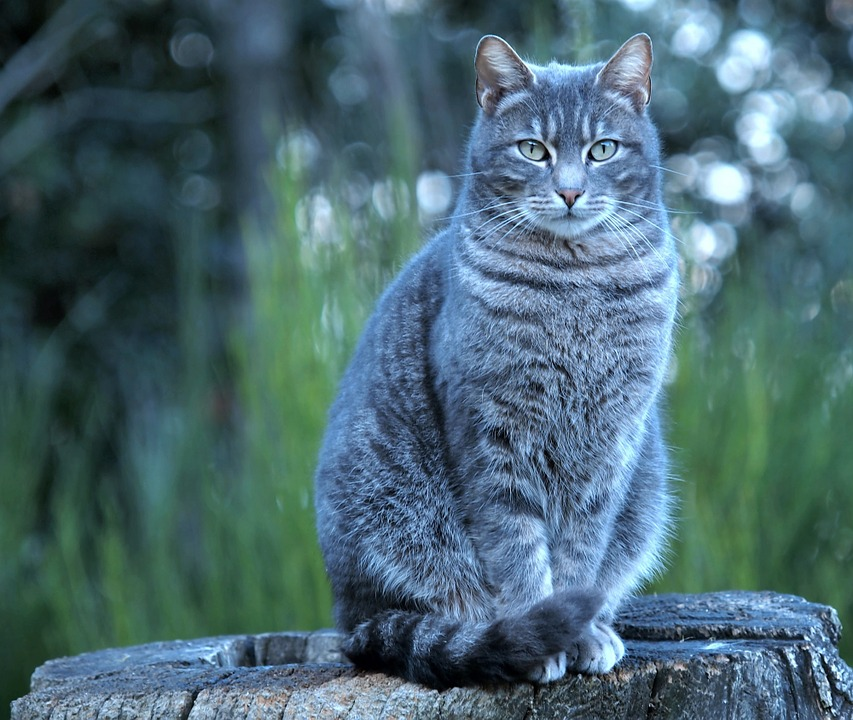
\includegraphics[height=6cm]{figures/cat.jpg}
          \vspace{0.5cm}

          \end{center}
      \end{minipage}
      \begin{minipage}{0.1\linewidth}
      \begin{center}

		 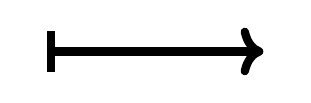
\begin{tikzpicture}
		 \node (a) at (0,0){};
		 \node (b) at (3,0){};
		 \draw[ |->,line width=3pt] (a) edge node [left] {} (b) ;
		 \end{tikzpicture}

         \end{center}
      \end{minipage} \hspace{0cm}
	\begin{minipage}{0.16\linewidth}
	\begin{center}
          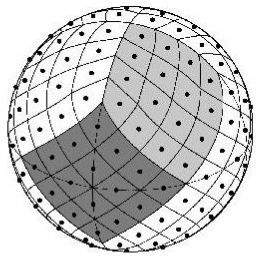
\includegraphics[height=5cm]{figures/sphere.png}


          \end{center}
      \end{minipage}
   \begin{minipage}{0.1\linewidth}
      \begin{center}

		 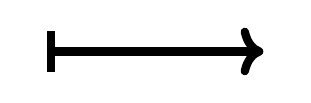
\begin{tikzpicture}
		 \node (a) at (0,0){};
		 \node (b) at (3,0){};
		 \draw[ |->,line width=3pt] (a) edge node [left] {} (b) ;
		 \end{tikzpicture}

         \end{center}
      \end{minipage} \hspace{0cm}
	\begin{minipage}{0.16\linewidth}
	\begin{center}
          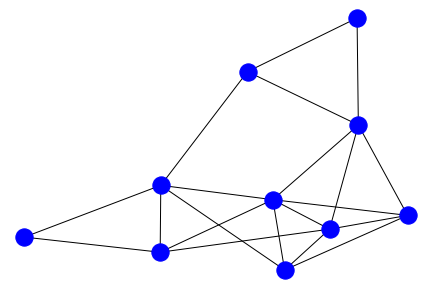
\includegraphics[height=5cm]{figures/graph.png}


          \end{center}
      \end{minipage}
   \begin{minipage}{0.1\linewidth}
      \begin{center}

		 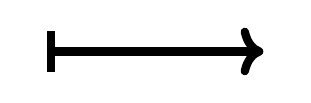
\begin{tikzpicture}
		 \node (a) at (0,0){};
		 \node (b) at (3,0){};
		 \draw[ |->,line width=3pt] (a) edge node [left] {} (b) ;
		 \end{tikzpicture}

         \end{center}
      \end{minipage} \hspace{0cm}
	\begin{minipage}{0.16\linewidth}
	\begin{center}
          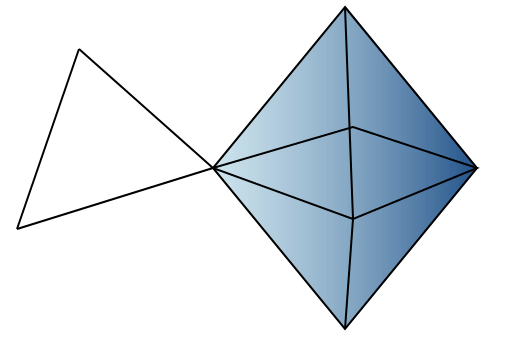
\includegraphics[height=5cm]{figures/high-order.png}


          \end{center}
      \end{minipage}
    \end{center}



\vspace{1cm}
 \begin{center}
\begin{minipage}{0.16\linewidth}
\vspace{-1cm}
		\begin{center}
		Convolutions:
		\\ local and shift-invariant
	\end{center}
      \end{minipage}
      \begin{minipage}{0.1\linewidth}
         \begin{center}
         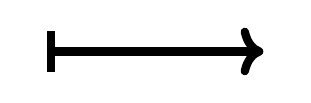
\begin{tikzpicture}
		 \node (a) at (0,0){};
		 \node (b) at (3,0){};
		 \draw[ |->,line width=3pt] (a) edge node [left] {} (b) ;
		 \end{tikzpicture}
	\end{center}
      \end{minipage}
	\begin{minipage}{0.16\linewidth}
	\vspace{-1cm}
         \begin{center}
        Convolutions:
		\\ local and group action-invariant
	\end{center}
      \end{minipage}
      \begin{minipage}{0.1\linewidth}
         \begin{center}
         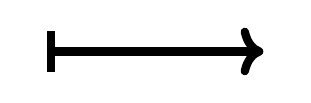
\begin{tikzpicture}
		 \node (a) at (0,0){};
		 \node (b) at (3,0){};
		 \draw[ |->,line width=3pt] (a) edge node [left] {} (b) ;
		 \end{tikzpicture}
	\end{center}
      \end{minipage}
	\begin{minipage}{0.16\linewidth}
	\vspace{-1cm}
         \begin{center}
          Convolutions:
		\\ localization-invariant
	\end{center}
      \end{minipage}
  \begin{minipage}{0.1\linewidth}
         \begin{center}
         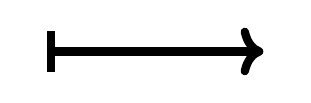
\begin{tikzpicture}
		 \node (a) at (0,0){};
		 \node (b) at (3,0){};
		 \draw[ |->,line width=3pt] (a) edge node [left] {} (b) ;
		 \end{tikzpicture}
	\end{center}
      \end{minipage}
	\begin{minipage}{0.16\linewidth}
	\vspace{-1cm}
         \begin{center}
          Convolutions:
		\\ localization-invariant
	\end{center}
      \end{minipage}


       \end{center}




    }
  \block{Basic building blocks of a space: simplices}{
		\begin{center}
		\vspace{-0.4cm}
		 \begin{minipage}{0.2\linewidth}
		 \begin{center}
          
\includegraphics[height=0.5cm]{figures/simp0.png}
          \end{center}
      \end{minipage} \hspace{0.5cm}
      \begin{minipage}{0.2\linewidth}
      \vspace{-0.5cm}
      \begin{center}
          
\includegraphics[height=3.5cm]{figures/simp1.png}
          \end{center}
      \end{minipage} \hspace{0.5cm}
	\begin{minipage}{0.2\linewidth}
	\vspace{-0.5cm}
	\begin{center}
          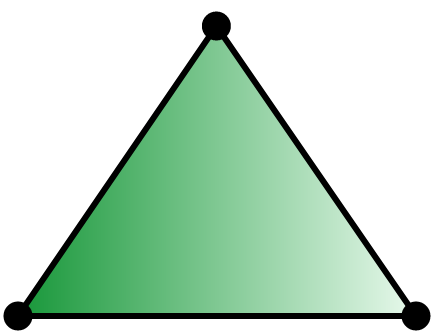
\includegraphics[height=3.5cm]{figures/simp2.png}
          \end{center}
      \end{minipage} \hspace{1.5cm}
      \begin{minipage}{0.2\linewidth}
      \vspace{-0.5cm}
      \begin{center}
          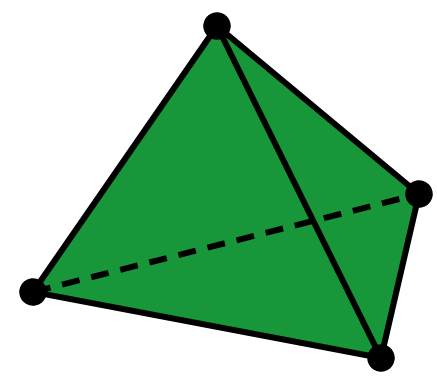
\includegraphics[height=3.5cm]{figures/simp3.png}
          \end{center}
      \end{minipage}
      \end{center}

      \begin{center}
      \vspace{-0.2cm}
      \begin{minipage}{0.2\linewidth}
		\begin{center}
		 0-simplex
	\end{center}

      \end{minipage}\hspace{0.5cm}
      \begin{minipage}{0.2\linewidth}
      \vspace{-0.2cm}
         \begin{center}
		 1-simplex
	\end{center}
      \end{minipage} \hspace{0.5cm}
	\begin{minipage}{0.2\linewidth}
	\vspace{-0.25cm}
         \begin{center}
		 2-simplex
	\end{center}
      \end{minipage} \hspace{1.5cm}
      \begin{minipage}{0.2\linewidth}
      \vspace{-0.2cm}
      \begin{center}
		 3-simplex
	\end{center}
      \end{minipage}
      \end{center}
   \vspace{-0.2cm}

    }


\block{Laplacians for simplicial complexes}{
The graph Laplacian can be extended to Laplacians for simplices of any dimension $k$ \cite{1}.
The $k$-Laplacian can be interpreted as a function propagating values of functions on the $k$-simplices.
These functions are called $k$-cochains, $x_k$.
\vspace{0.3cm}

\begin{center}
  \begin{minipage}{0.2\linewidth}
    \begin{center}
      $L_0$: Graph Laplacian\\
      $y_0=L_0x_0$
	\end{center}
  \end{minipage}
  \hspace{4.5cm}
  \begin{minipage}{0.2\linewidth}
    \begin{center}
      $L_1$: $1$-Laplacian\\
      $y_1=L_1x_1$
    \end{center}
  \end{minipage}
  \hspace{4.5cm}
  \begin{minipage}{0.2\linewidth}
    \begin{center}
      $L_2$: $2$-Laplacian\\
      $y_2=L_2x_2$
    \end{center}
  \end{minipage}
\end{center}

\begin{center}
  \begin{minipage}{0.2\linewidth}
    \begin{center}
      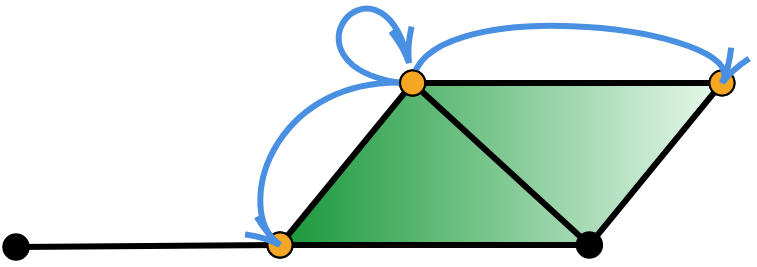
\includegraphics[height=4.8cm]{figures/glap0.png}
    \end{center}
  \end{minipage}
  \hspace{4.5cm}
  \begin{minipage}{0.2\linewidth}
    \begin{center}
      \vspace{1.5cm}
      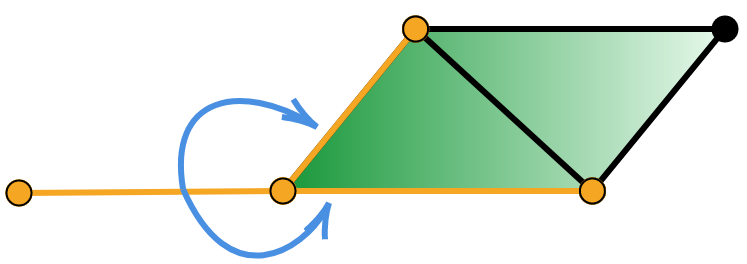
\includegraphics[height=4.58cm]{figures/glap1.png}
    \end{center}
  \end{minipage}
  \hspace{4.5cm}
  \begin{minipage}{0.2\linewidth}
    \begin{center}
      \vspace{0.1cm}
      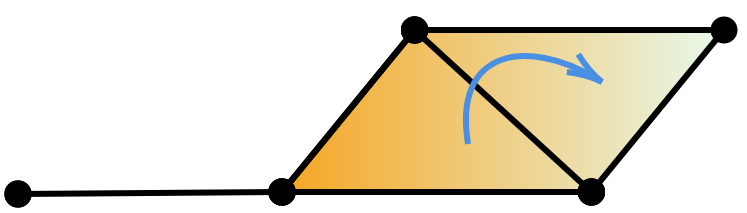
\includegraphics[height=3.9cm]{figures/glap2.png}
    \end{center}
  \end{minipage}
\end{center}
}


\block{Simplicial Neural Networks (SNNs)}{
\begin{center}
    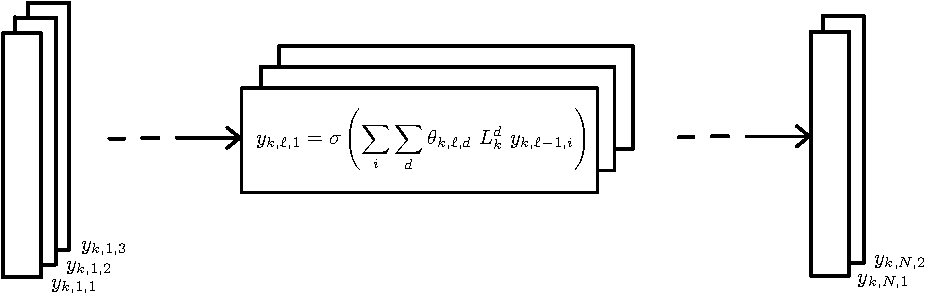
\includegraphics[width=0.87\linewidth]{figures/snn}
\end{center}
\begin{itemize}
    \item Linear cost: convolutions are sparse matrix-vector multiplications.
    \item $O(1)$ weights to be learned.
    \item $d$-localizing: no interaction between simplices that are more than $d$ hops apart.
\end{itemize}
}




  }

 \column{0.5}{


 \block{Coauthorship complex: from a bipartite graph to a complex}{

\vspace{0.5cm}

\begin{minipage}{0.2\linewidth}
 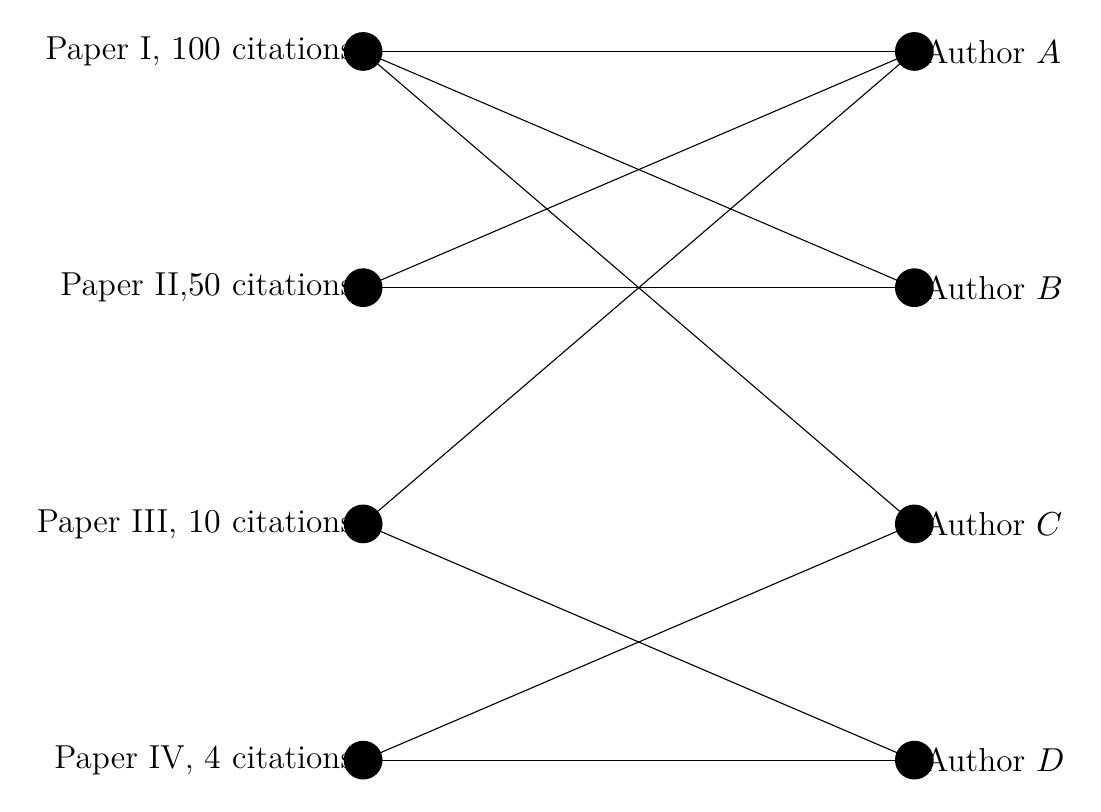
\begin{tikzpicture}[font=\scriptsize]
    \coordinate (I) at (0,0);
    \coordinate (II) at (0,-3);
    \coordinate (III) at (0,-6);
    \coordinate (IV) at (0,-9);

    \coordinate (A) at ($ (I) + (7,0) $);
    \coordinate (B) at ($ (II) + (7,0) $);
    \coordinate (C) at ($ (III) + (7,0) $);
    \coordinate (D) at ($ (IV) + (7,0) $);

    \fill[color=black] (I) circle (7pt);
    \fill[color=black] (II) circle (7pt);
    \fill[color=black] (III) circle (7pt);
    \fill[color=black] (IV) circle (7pt);
    \fill[color=black] (A) circle (7pt);
    \fill[color=black] (B) circle (7pt);
    \fill[color=black] (C) circle (7pt);
    \fill[color=black] (D) circle (7pt);

    \node[anchor=east] at (I) {\large Paper \MakeUppercase{\romannumeral 1}, \large $100$ citations};
    \node[anchor=east] at (II) {\large Paper \MakeUppercase{\romannumeral 2},\large  $50$ citations};
    \node[anchor=east] at (III) {\large Paper \MakeUppercase{\romannumeral 3}, \large  $10$ citations};
    \node[anchor=east] at (IV) {\large Paper \MakeUppercase{\romannumeral 4}, \large $4$ citations};

    \node[anchor=west] at (A) { \large Author $A$};
    \node[anchor=west] at (B) {\large Author $B$};
    \node[anchor=west] at (C) {\large Author $C$};
    \node[anchor=west] at (D) {\large Author $D$};

    \draw (I) -- (A);
    \draw (I) -- (B);
    \draw (I) -- (C);

    \draw (II) -- (A);
    \draw (II) -- (B);

    \draw (III) -- (A);
    \draw (III) -- (D);

    \draw (IV) -- (C);
    \draw (IV) -- (D);
  \end{tikzpicture}


\end{minipage}%
\hspace{14cm}
\begin{minipage}{0.2\linewidth}

  \begin{tikzpicture}[font=\scriptsize]
    \coordinate (A) at (0,0);
    \coordinate (B) at (9,0);

    \coordinate (C) at ($ (A) + (275:6) $);
    \node[anchor=north] at (C) {\large $100$};

    \coordinate (D) at ($ (B) + (265:6) $);
    \node[anchor=north] at (D) {\large $50$};

    \draw[dashed] (A) -- (C) -- (B);
    \draw[dashed] (A) -- (D) -- (B);


    \coordinate (AA) at ($ (A) + (0, -8.5) $);
    \coordinate (BB) at ($ (B) + (0, -8.5) $);

    \fill[color=black] (A) circle (7pt);
    \fill[color=black] (B) circle (7pt);
    \fill[color=black] (AA) circle (7pt);
    \fill[color=black] (BB) circle (7pt);

    \draw (A) -- (B);
    \draw (AA) -- node[below, align=center] {\large $1$-cochain \\\\ \large $150=100+50$} (BB);

    \node[anchor=east] at (A) {\large $A$};
    \node[anchor=west] at (B) {\large $B$};
    \node[anchor=east] at (AA) {\large $A$};
    \node[anchor=west] at (BB) {\large $B$};

  \end{tikzpicture}

\end{minipage}
\hspace{1cm}
\begin{minipage}{0.2\linewidth}

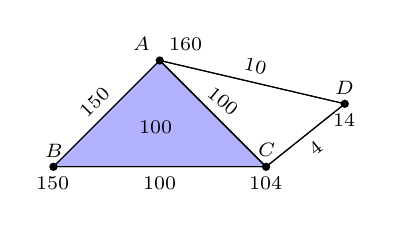
\begin{tikzpicture}[font=\scriptsize] % Dirty last minute TikZ with calc cheating and hardcoding.
  \coordinate (b) at (0,0);
  \coordinate (c) at (2.7,0); %($ (b) + (20:2) $);
  \coordinate (a) at (1.35,1.35); %($ (b) + (80:2) $);
  \coordinate (d) at (3.7,0.8); %($ (c) + (30:2) $);

  \draw[twosimp] (a) -- (b) -- (c) -- cycle;
  \draw (a) -- (d) -- (c) -- cycle;
  \fill[color=black] (a) circle (1.5pt);
  \fill[color=black] (b) circle (1.5pt);
  \fill[color=black] (c) circle (1.5pt);
  \fill[color=black] (d) circle (1.5pt);

  \draw (a) -- (b) node [midway,sloped,above] {$150$};
  \draw (a) -- (c) node [midway,sloped,above] {$100$};
  \draw (b) -- (c) node [midway,sloped,below] {$100$};
  \draw (c) -- (d) node [midway,sloped,below] {$4$};
  \draw (a) -- (d) node [midway,sloped,above] {$10$};
  %\node () at ($ (b) + (50:1.15) $) {$100$};
  \node () at (1.3,0.5) {$100$};
  
  \node[anchor=south west] at (a) {$160$};
  \node[anchor=south east] at (a) {$A$};
  
  \node[anchor=north] at (b) {$150$};
  \node[anchor=south] at (b) {$B$};

  \node[anchor=north] at (c) {$104$};
  \node[anchor=south] at (c) {$C$};

  \node[anchor=north] at (d) {$14$};
  \node[anchor=south] at (d) {$D$};
\end{tikzpicture}

\end{minipage}


\vspace{0.5cm}

}



    \block{Predicting missing citations on the coauthorship complex}{
\begin{center}
\Large{\textbf{Data}}
\end{center}
\begin{center}
Coauthorship complexes are built from the Semantic Scholar dataset \cite{2} where missing citations are introduced at random on the $k$-cochains ($k=1,2,3$) at five rates: $10\%, 20\%,  30\%, 40\%$, and $50\%$.

\end{center}
\vspace{0.5cm}
\begin{center}
\begin{minipage}{0.2\linewidth}
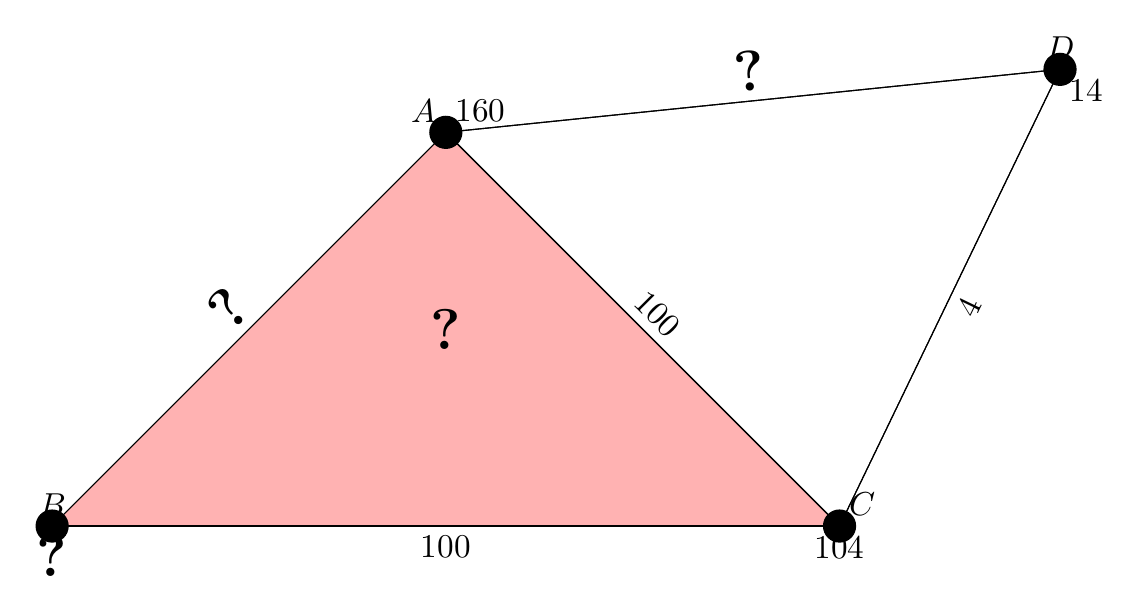
\begin{tikzpicture}[font=\scriptsize] % Dirty last minute TikZ with calc cheating and hardcoding.
  \coordinate (b) at (0,0);
  \coordinate (c) at (10,0); %($ (b) + (20:2) $);
  \coordinate (a) at (5,5); %($ (b) + (80:2) $);
  \coordinate (d) at (12.8,5.8); %($ (c) + (30:2) $);

  \draw[twosimpred] (a) -- (b) -- (c) -- cycle;
  \draw (a) -- (d) -- (c) -- cycle;
  \fill[color=black] (a) circle (6pt);
  \fill[color=black] (b) circle (6pt);
  \fill[color=black] (c) circle (6pt);
  \fill[color=black] (d) circle (6pt);

  \draw (a) -- (b) node [midway,sloped,above] {\huge \textbf{?}};
  \draw (a) -- (c) node [midway,sloped,above] {\large $100$};
  \draw (b) -- (c) node [midway,sloped,below] {\large $100$};
  \draw (c) -- (d) node [midway,sloped,below] {\large $4$};
  \draw (a) -- (d) node [midway,sloped,above] {\huge \textbf{?}};
  %\node () at ($ (b) + (50:1.15) $) {$100$};
  \node () at (5,2.5) {\huge \textbf{?}};
  
  \node[anchor=south west] at (a) {\large $160$};
  \node[anchor=south east] at (a) {\large $A$};
  
  \node[anchor=north] at (b) {\huge \textbf{?}};
  \node[anchor=south] at (b) {\large $B$};

  \node[anchor=north] at (c) {\large $104$};
  \node[anchor=south west ] at (c) {\large $C$};

  \node[anchor=north west] at (d) {\large $14$};
  \node[anchor=south] at (d) {\large $D$};
\end{tikzpicture}

\end{minipage}
\end{center}
\vspace{-1.5cm}
\begin{center}
\Large{\textbf{First Results}}
\end{center}
\begin{center}
Mean accuracy $\pm$ standard deviation over 5 samples in imputing missing citations.
\vspace{0.5cm}

\begin{minipage}{1\linewidth}
\begin{center}
  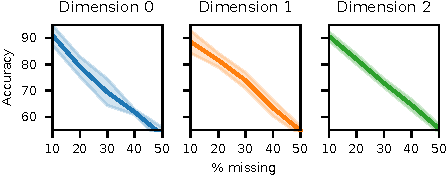
\includegraphics[height=14cm]{figures/performance_accuracy.pdf}
 \end{center}
 \end{minipage}
\vspace{0.5cm}
Performance of baselines: mean accuracy $\pm$ standard deviation over 5 samples for $30\%$ missing citations.
\vspace{0.5cm}
\begin{minipage}{1\linewidth}
\begin{center}
\begin{tikzfigure}
\large{\begin{tabular}{lrrr}
      \hline
      Method & Dimension 0 & Dimension 1 & Dimension 2 \\
      \hline
      Global Mean & $3.30\pm0.82$ & $5.75\pm1.28$ & $2.96\pm0.49$ \\
      Global Median & $7.78\pm2.70$ & $10.44\pm1.00$ & $12.50\pm0.63$ \\
      Neighbors Mean & $11.88\pm5.29$ & $24.15\pm1.85$ & $27.38\pm1.18$ \\
      \hline
    \end{tabular}}
    \vspace{9pt}
\end{tikzfigure}
\end{center}
\end{minipage}

\begin{center}
\textbf{Code: \url{https://github.com/stefaniaebli/simplicial_neural_networks}}
\end{center}

\end{center}

}

    \block{References}{
     % \begin{center}%\mbox{}\vspace{-\baselineskip} % This bullshit is workaround for certain versions of tikzposter.
        % More info at https://tex.stackexchange.com/questions/243665/bibliography-printing-without-numbers-tikzposter
     %\printbibliography[heading=none]
%\small{ Reconstruction and simulation of neocortical microcircuitry, Markram et al.\, Cell, 163, 2, 456--492, 2015, Elsevier.}
\begingroup
\renewcommand{\section}[2]{}%
\small
\begin{thebibliography}{1}


\bibitem{hor} D.\ Horak and J.\ Jost, {\em Spectra of combinatorial Laplace operators on
  simplicial complexes}, Adv.\ in Math.\, 2013.
\bibitem{sem} W.\ Ammar et al.\ , {\em Construction of the Literature Graph in Semantic Scholar}, \url{https://www.semanticscholar.org/paper/09e3cf5704bcb16e6657f6ceed70e93373a54618}.


\end{thebibliography}
     %\end{center}
\endgroup
      %\scriptsize Artist's depiction of microcircuit column by Nicolas Antille, Blue Brain
     % Project. Soap bubble picture by Wikipedia user Rror,2009
      %CC-BY-SA-3.0.

    }
  }
\end{columns}

\end{document}
